\section{Literature Review}
\subsection{Existing Systems}
Ticket vending machines (TVMs) have become increasingly popular over the past several years, being used to replace manned ticketing kiosks in a variety of sectors. Whilst buying a train ticket from a machine has been a possibility for decades, it is only relatively recently that a single touchscreen interface has become the norm for these machines. However,as discussed previously,  research into train ticket vending efficiency has suggested a customer preference of a manned kiosk over a TVM. Studies attempting to determine the reasoning behind this preference identified several key issues with the current user interfaces (UI) obtained via passenger feedback (ref). Several of the issues identified (TransportFocus 2016) have been summarised below:

\begin{itemize}
	\item Difficulty of interacting with touchpad - customers found that the touchpad was generally unresponsive and often poorly calibrated, making selecting options on screen difficult
	\item Too much jargon - customers experienced confusion over off-peak and peak times and when a travel card could be used. Ages applicable to child fares were also often not shown.
	\item Sheer volume of information- customers felt the amount of information displayed on the screen was overwhelming and made it difficult to decide where to press.
	\item Visibility of key options - Information boxes to the side and bottom of screens were often not seen by passengers.
	\item Poor choice of colour scheme- for example, customers found that information in yellow writing was not readily visible and that a colour scheme of blue and green did not provide enough contracts to easily read on the screen.
	\item Intervention by staff still required - In some cases information about routes and restrictions was not provided, instead instructions were given to ask a member of staff for information.
\end{itemize}


In the following section, two existing UIs designed for TVMs will be examined in order to determine the current prevalence the above issues in the UK and to identify further barriers to the usability of TVMs. There has been much research in the area of improving usability of ticketing machines across a range of sectors and both good and bad elements of interface design will be identified in existing models in order to help determine the requirements for an improved approach to train ticket vending.
In the UK, there are two particular designs of ticket machine that are utilised by the majority of train operators. These are the Scheidt \& Bachmann Ticket Xpress and the Shere FASTticket. The UI of each machine has a different livery for each individual train operator however the underlying UI is essentially the same. An example of each of these widely used machines will be analysed to determine both positive and negative aspects of their UIs from a user centred design perspective.

\subsubsection{Shere FASTticket}
The example of the Shere FASTticket machine discussed here is a Virgin Trains ticket machine found at Birmingham New Street Station. In terms of the physical machine, the UI consists of a 15 inch touchscreen, chip-and-pin keypad and a tray into which the printed tickets are delivered. There are two variations of the machine, one which takes credit/debit card only and one which also takes cash. Nearly 60\% of purchases in the UK still being undertaken in cash (Consult Hyperion, 2013) and it was anecdotally noted at both times at which the machine was examined (once at peak time and once at an off-peak time), there were queues for both the manned ticketing office and the machines that take cash whilst several card-only machines were still free. This would suggest that consumers prefer to have the option to pay with cash; this is a design feature that adds choice to the process without impacting on the usability of the system as the customer will likely have decided in advance on their preferred method of payment. 

The main UI of the Shere FASTticket is the touch screen via which the majority of actions are performed. The initial screen on approaching the machine is shown in Figure \ref{fig:avoidQueues}. 

\begin{figure}[h]
	\centering
	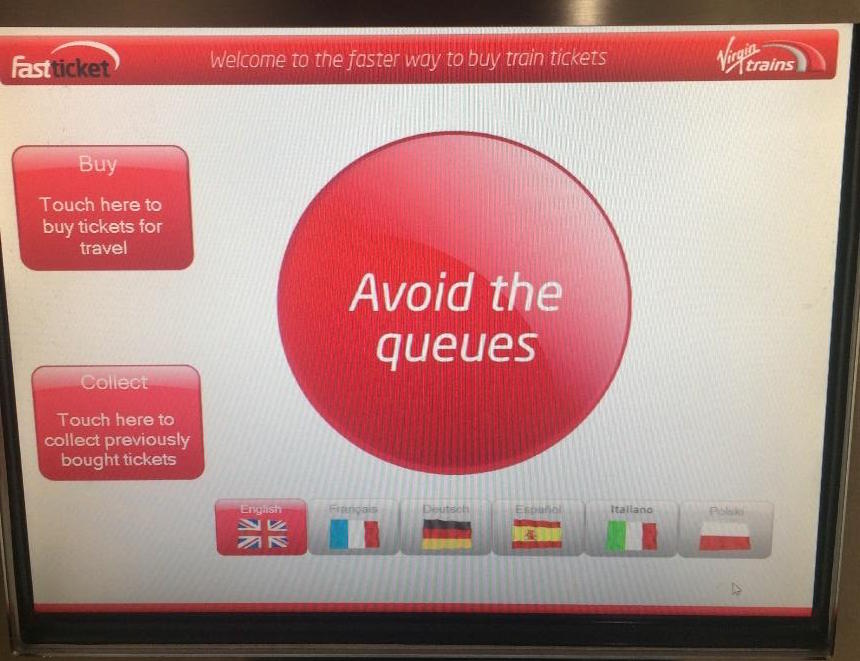
\includegraphics[width=0.5\linewidth, angle=0, origin=c]{images/image02}
	\caption{To Do}
	\label{fig:avoidQueues}
\end{figure}

The screen in Figure \ref{fig:avoidQueues} provides several options:
\begin{enumerate}
	\item Buy tickets for travel
	\item Collect pre-bought tickets
	\item Choose language – languages represented by country flags
\end{enumerate}

This simple starting point requires the user to choose between two options, this is an easy decision as a user will be aware of whether they have pre-booked a ticket or not. The use of flags to represent the languages is easy to understand however it does mean that the language selection is limited to the six languages specified. The large red circle in the centre of the screen has no function, this has the potential to be confusing for those who are using the machine for the first time. The screen does however follow good design principles in that it provides only the key information required to make this first decision and has a clear method of changing language which does not require any knowledge of the default language, the issue of presenting language options is discussed in more detail later in the report. On the other hand, the largest feature of the screen, a “big red button” has no function and detracts from the usability of the system by providing unnecessary distraction. 

In order to demonstrate the usability of the UI, a typical scenario of buying a ticket was enacted. The users in this scenario are a pair of students wishing to buy one way tickets to Southampton at 7pm on a week day using their 16-25 rail-cards to get a discount. They select the option to buy tickets from the welcome screen and are taken to the screen shown in Figure \ref{fig:destination}.

\begin{figure}[h]
	\centering
	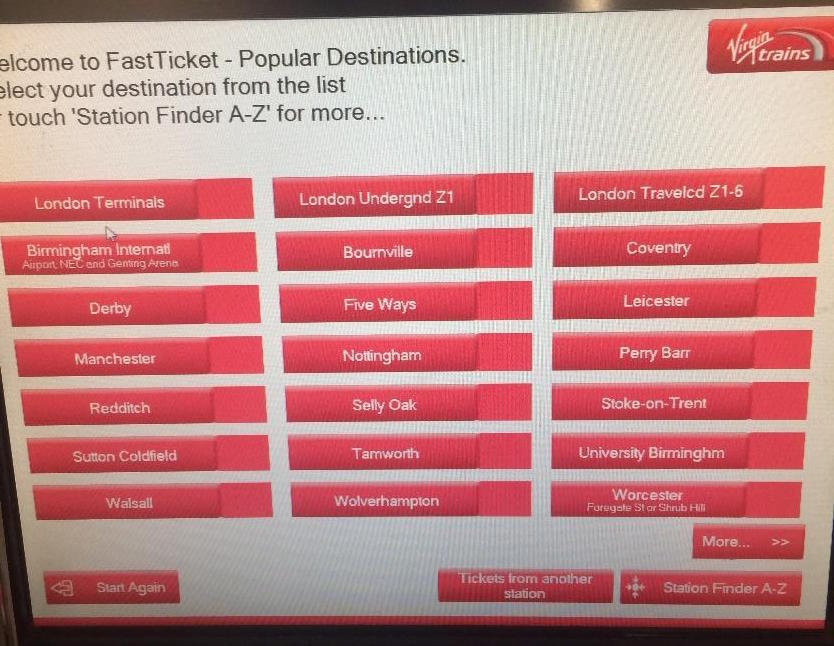
\includegraphics[width=0.5\linewidth, angle=0, origin=c]{images/image06}
	\caption{To Do}
	\label{fig:destination}
\end{figure}

This screen contains 21 different “popular destinations”. If, as in this scenario, the user wishes to travel to a different destination, they can use the Station Finder A-Z button in the bottom right corner. The functionality to buy tickets for a different starting station also exists and is accessed by pressing the button “Tickets from another station” however this is not required in this case. There is also a “start again” button to return to the welcome screen. For a first time user of this system, or someone with a learning disability or low level of technical knowledge, the sheer amount of information and optionality on this page impacts the usability of the UI. The theory of choice overload becomes relevant here; it has been shown that too large a set of possible choices can lead to choice overload which results in reduced user satisfaction (Bollen et al, 2010).

The option of choosing a different station comes only in the form of a small button that is difficult to distinguish from the other options on the screen, the instructions on using the UI also do not stand out on the screen and were not noticed initially. As discussed previously, customers have stated that buttons at the bottom or side of the screen are often missed and reduce the usability of the UI.  In general, searching through a list of possible destinations is impractical and unlikely to encourage an impatient customer to make use of the ticketing machine again. For the scenario described previously, the students take the time to read through the popular destinations, discover that Southampton is not present and select the Station Finder A-Z option to reach the screen shown in Figure \ref{fig:keyboard}. 

\begin{figure}[h]
	\centering
	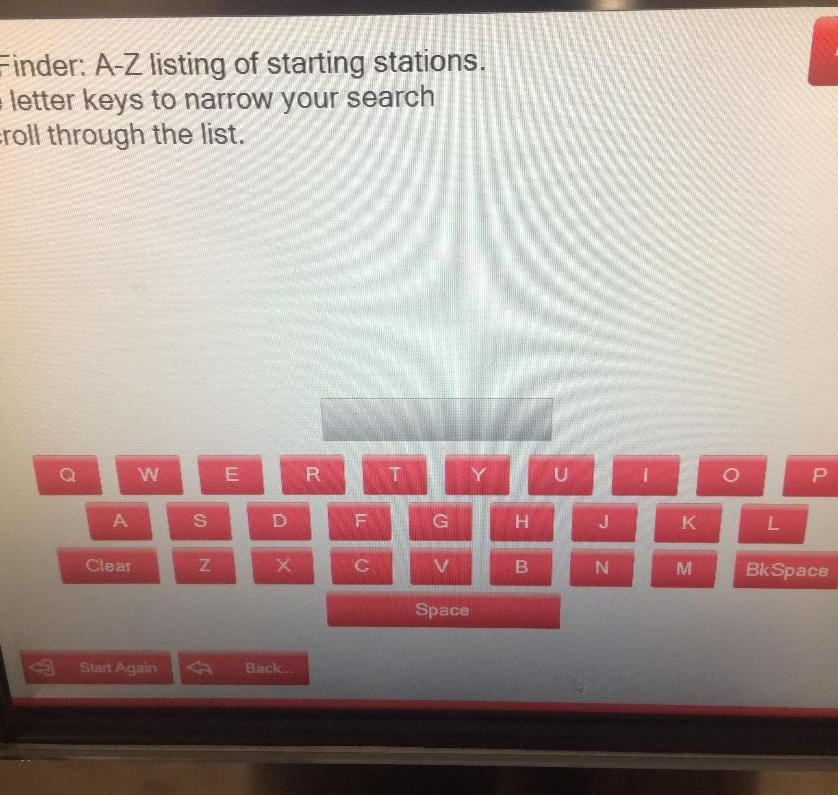
\includegraphics[width=0.5\linewidth, angle=0, origin=c]{images/image04}
	\caption{To Do}
	\label{fig:keyboard}
\end{figure}

The user must type in the required destination on a QWERTY keyboard; although it has been shown that the elderly find an alphabetic keyboard more intuitive (ref), as time progresses it is likely that the majority of users will be familiar with the layout of a QWERTY keyboard and so this seems like a sensible design decision.

Once the destination has been selected, a selection of possible ticket types are displayed as shown in Figure \ref{fig:peaks}.  Again choice overload becomes an issue along with a large amount of train ticket jargon such as off-peak, anytime, day return etc which may well not be intuitive to a first time user.. The addition of railcards and additional passengers is fairly straightforward, the railcards option is selected and the required railcard to add is chosen from a screen of the different types of card shown in Figure \ref{fig:railcard}. The number of passengers is selected from a choice of 1 to 8 passengers as shown in Figure \ref{fig:passengers}. In terms of the issues raised in previous studies, the relevant age limit for a child ticket is stated on the number of passengers screen (Figure \ref{fig:passengers}), however the text is small and difficult to read given the glare produced by the screen.

\begin{figure}[h!]
	\centering
	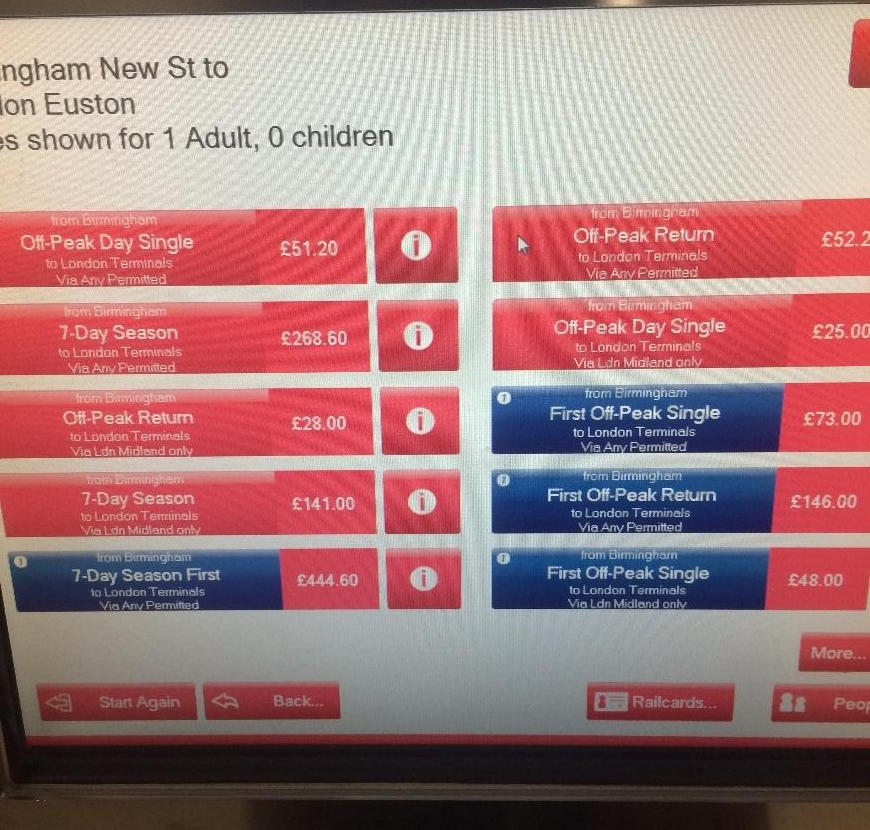
\includegraphics[width=0.5\linewidth, angle=0, origin=c]{images/image01}
	\caption{To Do}
	\label{fig:peaks}
\end{figure}

\begin{figure}[h!]
	\centering
	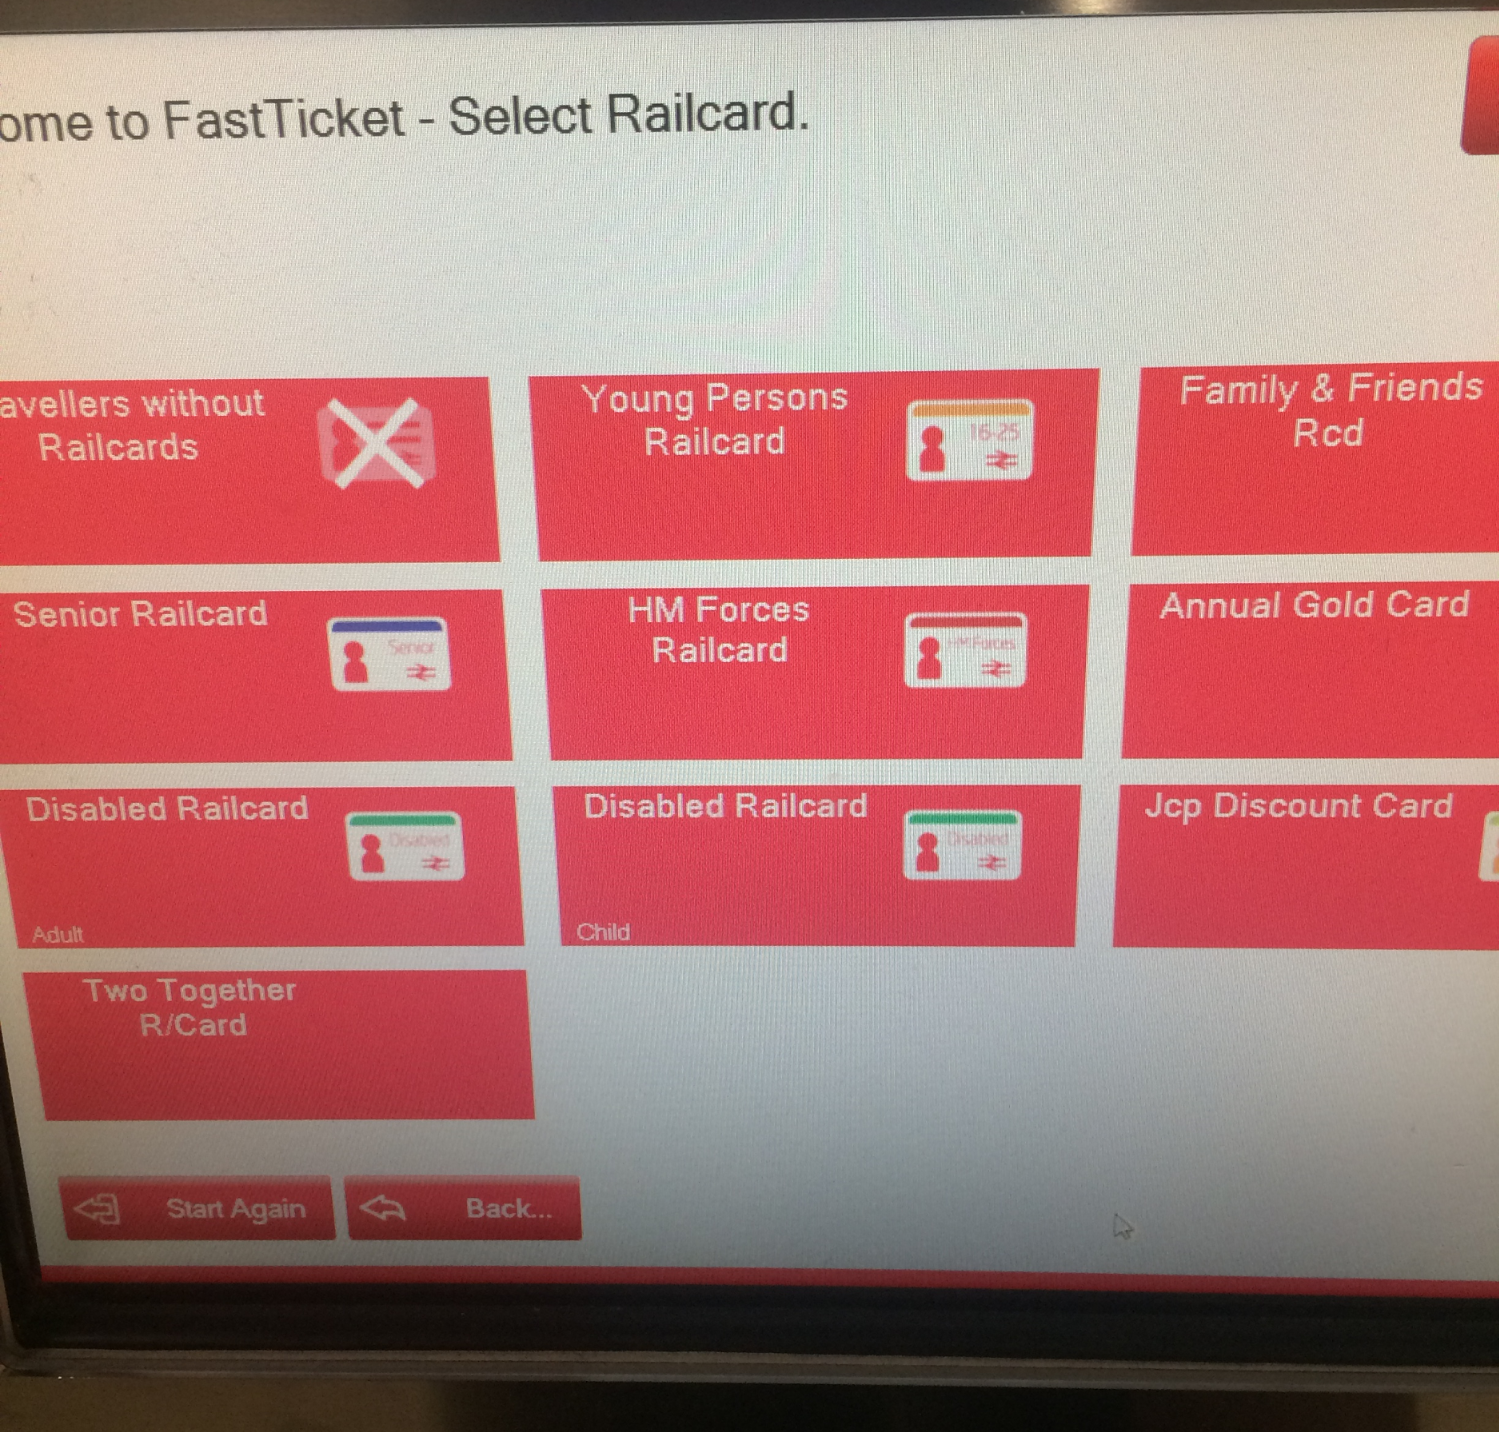
\includegraphics[width=0.5\linewidth, angle=0, origin=c]{images/image05}
	\caption{To Do}
	\label{fig:railcard}
\end{figure}

\begin{figure}[h!]
	\centering
	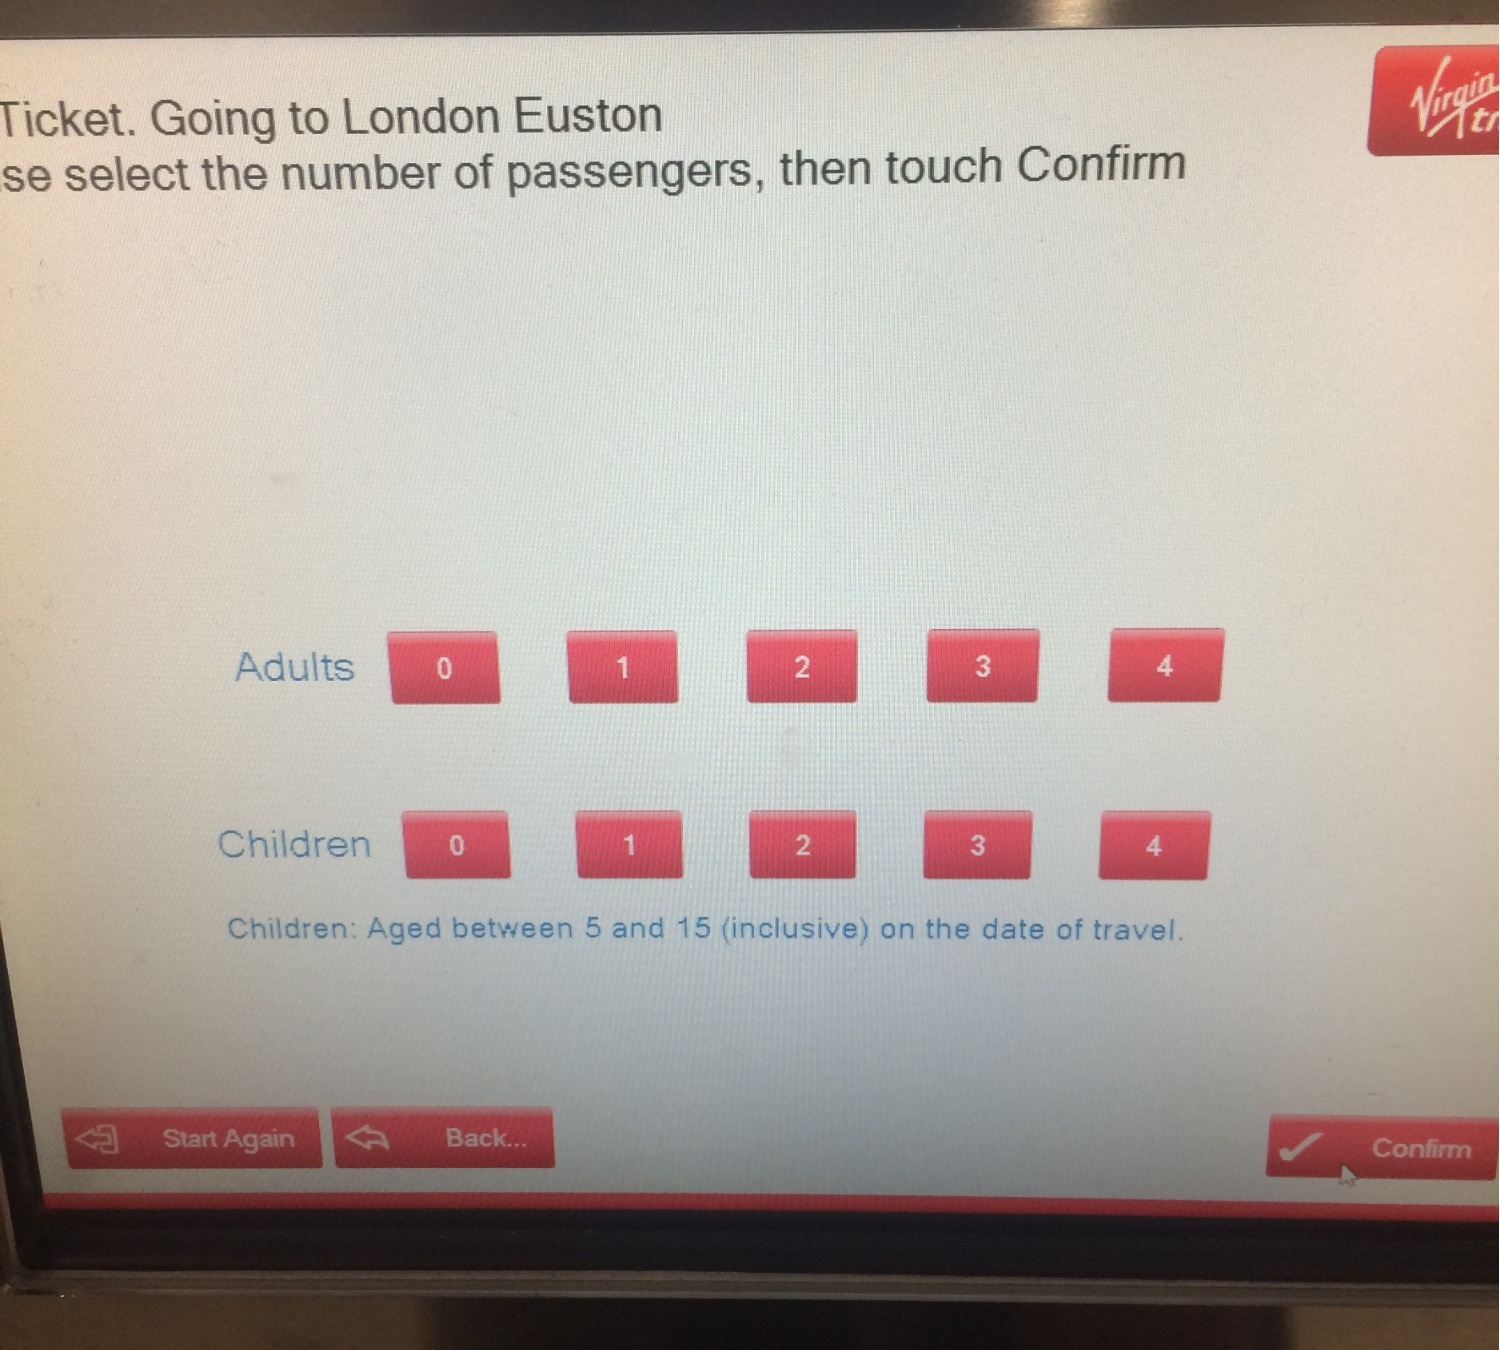
\includegraphics[width=0.5\linewidth, angle=0, origin=c]{images/image00}
	\caption{To Do}
	\label{fig:passengers}
\end{figure}

\newpage
Overall, several of the issues identified by passengers are shown to be prevalent in this particular UI:
\begin{itemize}
	\item Jargon is used without being easily explained
	\item Information overload
	\item Buttons to the side and bottom of the screen are not easily found
	\item Off peak timings and child age restrictions not immediately obvious
\end{itemize}
Additional issues were also identified:
\begin{itemize}
	\item Choice overload
	\item Excessive number of steps to achieve goal
	\item Redundant objects on screen are misleading
\end{itemize}

\subsubsection{Scheidt \& Bachmann}

Similar issues were found in the UI for the Scheidt \& Bachmann Ticket Xpress, here a machine with the London Midland livery was examined. The main issue here was again choice and information overload. In contrast to the FASTticket design, there is no welcome screen, interaction commences with a screen of popular journeys demonstrated in Figure \ref{fig:midlandSelection}. 

\begin{figure}[h!]
	\centering
	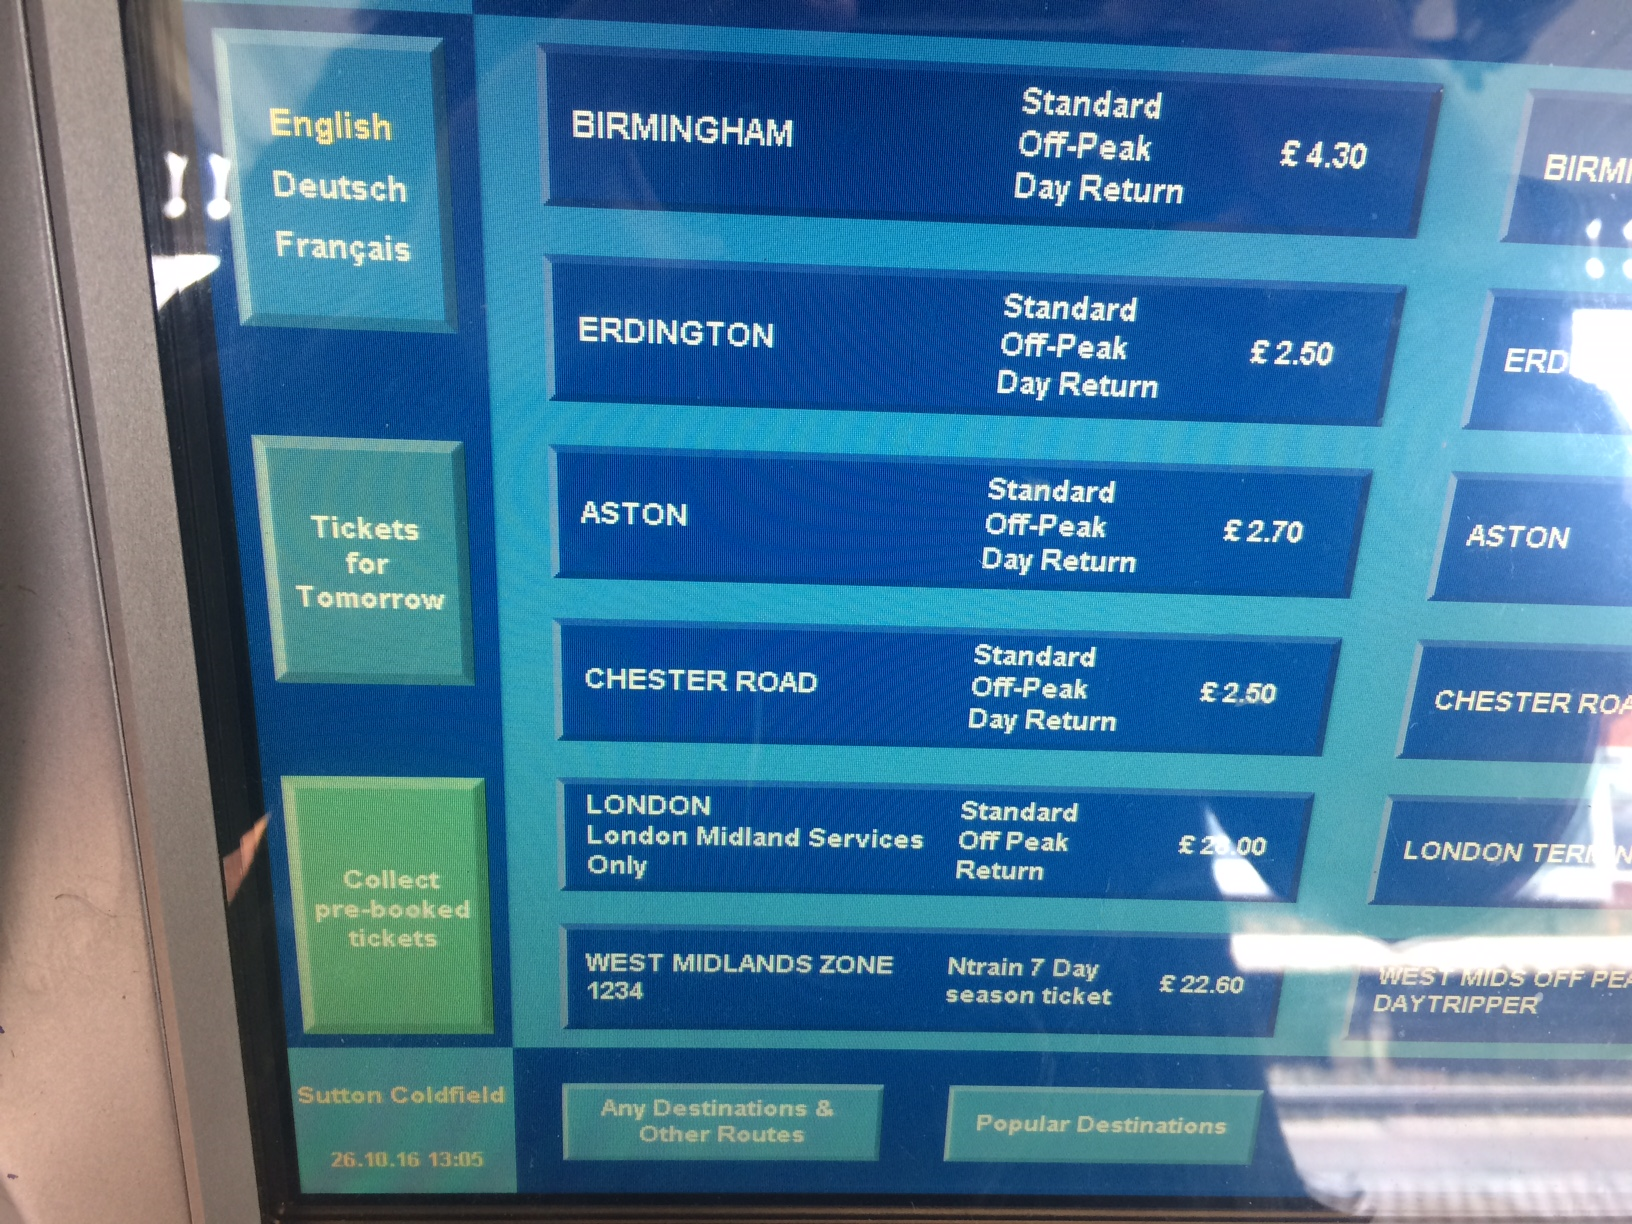
\includegraphics[width=0.5\linewidth, angle=0, origin=c]{images/image08}
	\caption{To Do}
	\label{fig:midlandSelection}
\end{figure}

\begin{figure}[h!]
	\centering
	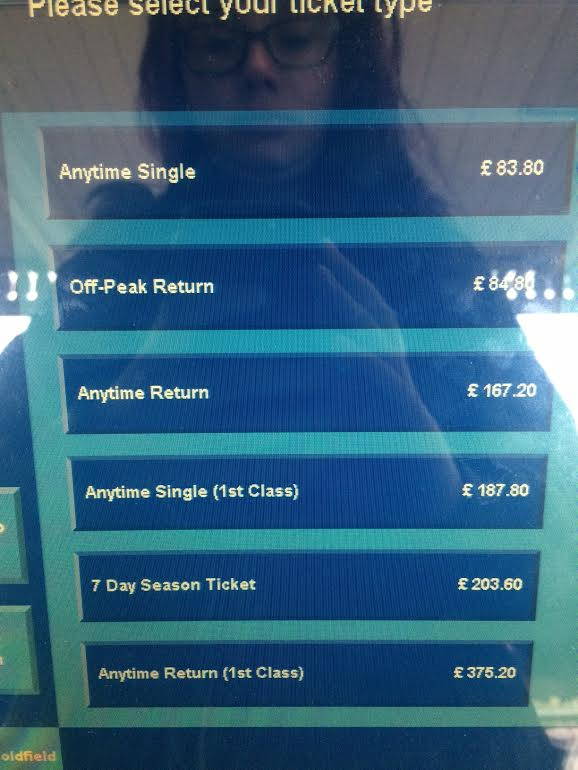
\includegraphics[width=0.5\linewidth, angle=0, origin=c]{images/image07}
	\caption{To Do}
	\label{fig:midlandType}
\end{figure}

Whilst there are few redundant graphics on the screen, in comparison to the previous design, there are options to perform several different actions from this screen. The option to collect pre-booked ticket exists, however the button to do so is located in the corner of the screen, with small white text on a pale green background. The issues of poorly readable text and buttons at the side of the screen being missed were raised in previous studies and are clear design flaws of this UI. When selecting a station other than those on the initial screen, the name of the station must be typed in, this time on an alphabetic keyboard. As discussed previously, this is less intuitive for the majority of users and increases the time taken to purchase a ticket. Ambiguity in ticket types is also an issue, no indication could be found of the eligible times for an off peak ticket. On the other hand the addition of rail-cards and passengers once a ticket has been selected is again fairly intuitive, the relevant age limit for a child ticket is clearer on this UI than in the previous case.

It is apparent from the above case studies that there are still many design issues with train ticketing UIs and that little has been done practically to address the concerns of customers determined in previous studies. 

\subsection{Other Existing Approaches to Self Service Machines}
Upon further research, it became apparent that several of the issues identified with self service machines in the transport sector are in fact common to many other sectors. One sector in which large amounts of time and money have been spent on interface improvement is in self-service checkout machines in supermarkets. Similar to TVMs at railway stations, these machines have been introduced to reduce both staffing costs and queueing times, however unlike the rail industry, where rail operators each claim ownership of specific lines, the supermarket sector is fiercely competitive with significant financial investment into improving the shopping experience in an attempt to win customers from their rivals; a study by (ref) identified a positive correlation between a good user experience of self service machines and customer loyalty. Several aspects of the Tesco self service checkout system are examined below in order to determine positive design ideas that could be applied to a train ticketing interface. The first aspect of the user interface that is of particular interest is the search method for items that do not have a bar-code, i.e. loose fruit and vegetables and bakery goods. As shown in Figure \ref{fig:supermarketCheckout}, the look up options for these items are presented in groups which make the items easy to classify. The options are presented as large folder shaped buttons, an indication that these are interactive buttons to press. The use of images in addition to text improves usability as users can determine the required category more quickly. This categorisation of items into an easily searchable format is a design element that could be explored in the context of purchasing train tickets, specifically in the selection of rail-cards, additional passengers and route specifics. The use of images, and the resulting ability to expedite searching for a required item is also an idea to be considered for TVMs , for example for tourists wishing to visit popular areas by train, an image of an easily recognisable local attraction could decrease search time on a “popular destinations” screen like those seen in the existing systems.

%\begin{figure}[h!]
%	\centering
%	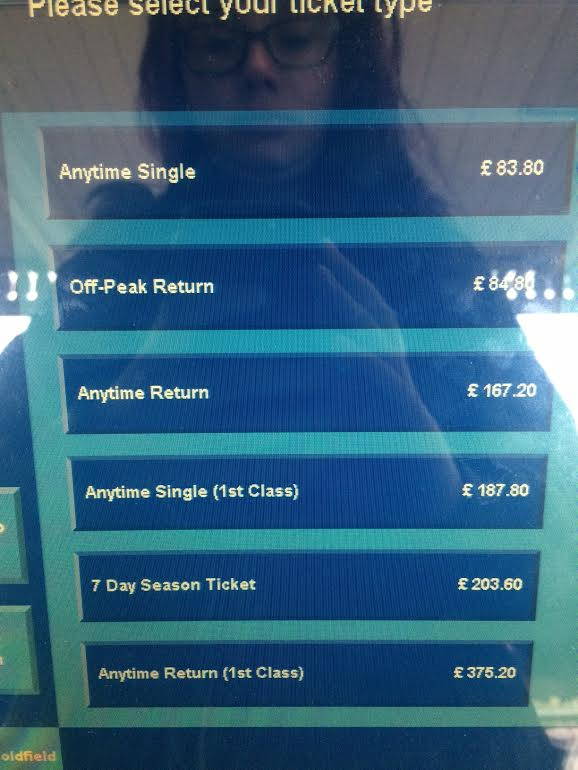
\includegraphics[width=0.5\linewidth, angle=0, origin=c]{images/image07}
%	\caption{To Do}
%	\label{fig:supermarketCheckout}
%\end{figure}

Modern self checkout machines also frequently make use of tutorial videos in order to aid in the use of the machine, For example, as shown in figure x, part of the screen consists of an animation indicating how to scan items and where to place them once they have been scanned. In this way. This is far more efficient that listing textual instructions which can be easily missed or misunderstood by the user. 

Self-checkout machines still have several design flaws however the majority are not relatable to vending train tickets, for example malfunctions with the scales tracking item weights and the need for a staff member to check IDs for the purchase of alcohol. They do however often present a large number of possible operations on one screen, giving the potential for choice overload, a design issue that should be avoided where possible.

\subsection{Ticket Machine Interface Design in Literature}

\subsubsection{Approaches to Ticket Machine Redesigns}
The issue of H.C.I. design within self-service rail ticketing machines has been tackled by different groups around the world, resulting in a variety of approaches that attempt to solve the problem. The employed strategies highlight existing U.I. shortfalls and establish a new focus on how the user interacts with the interface for the re-design. Subsequently a new set of methods are put forward to tackle the U.I. problem. These alternative approaches investigate two particular areas, the first is the use of colour and graphical representation, and the second is interface simplification; reducing the number of options and requesting user input sequentially.


\subsubsection{Colour and Graphical Representation}
The use of graphics and colour are fundamental in creating a successful UI but it should be used sparingly so as not to overwhelm the user. Sandnes (2010) discusses how Taiwan Rail’s first heuristic highlights the importance of using graphical elements but only when they assist the user. Trivial graphics may lead to distraction by crowding the screen and impacting the user’s performance at completing the task. Over use of colour and high contrast may introduce confusion rather than highlight important aspects since no one colour stands out. Conversely, low contrast screens inhibit a user’s understanding of the interface and gives a lack of weight to certain elements,  Norman (2013) describes how sufficient visibility of U.I. controls is required in order for a user to assess the situation and make an informed decision to progress forward. It is therefore a fine balance in which sufficient contrast should be given through a limited set of colours (Sandnes, 2010). 

In addition to limiting the range of colours, the chosen colours must be readable by those who are visually impaired or suffer from colour blindness since ticketing machines should be designed for the widest array of users. Globally the prevalence of colorblindness is quite high and is therefore an important aspect when designing the colour scheme of a UI system (Okabe, M, 2008). Okabe, M (2008) states that ‘One in twelve Caucasian (8\%), one in 20 Asian (5\%), and one in 25 African (4\%) males are so-called "red-green" colorblind.’. To overcome this, the UI colour scheme can be designed in one of two ways to give more differentiation to elements; firstly by using patterns (Joshua Johnson, 2010), and secondly by using a colour blind barrier-free colour pallet (Okabe, M, 2008). The use of patterns such as hatching can help to separate two elements even if they are perceived to be the same colour by the user, this can be taken further through the use of edge stokes and shadows within button selections, in turn adding more distinction between elements (Joshua Johnson, 2010). This approach should not be a replacement for colour however, but instead be used in addition to a colourblind pallet Figure 10. A key component of the pallet is to use ‘warm’ and ‘cool’ colours alternately; two of the same type should be avoided. Okabe, M, (2008) also highlights that the the use of the colour red should be used with caution, especially for displaying important information. The vividness can make it appear black to those who are colourblind, as such red and black should not be used in conjunction with one another.

Figure 10 colour blind pallet.

The choice of font in the U.I. is also an important aspect. Scripts that use thin lines such as ‘Times’ or ‘New York’ can pose difficulties for readers, whereas bold fonts ‘Arial’ or ‘Helvetica’ can be perceived more easily (Okabe, M, 2008). The amount of text on screen should also be taken into account, similar to a large range of colour, the vast amount of text can introduce confusion to the U.I.. An approach to overcome this is to use graphics as they can be an alternative to words, Sandnes (2010) explores how choosing a single or return ticket can be portrayed using graphical arrows, not only to reduce text in this example but to also reduce ambiguity. Since languages can express the same thing with different words, a level of uncertainty can be introduced. The UK terms for “single” and “return” would be written as  “one-way” and “roundtrip” in the US. The use of a picture can however reduce ambiguity since an image can help to explain the ticket type at a glance, this method is used by the swiss rail company Figure 11. It has also been noted that the direction of a single trip should read in the same direction as the language of the user (Sandnes, 2010) such that someone from the UK would expect to see an arrow from left to right for a “single” ticket.


FIG 11 graphics Swiss Rail Company


Lee (2012) introduces the idea of using graphics to help identify certain location within London, in Figure 12 Big Ben is used as a graphical image to help portray to the user that this button will give them options to choose stations near to the landmark without needing to know the name of the stations themselves. Landmarks used alongside the location name could help to make journey decisions easier for the user. It is also helpful for tourists as identifying buttons with visual landmarks is quicker and more accurate than choosing place names Lee (2012). This ties into one of Taiwan Rail’s heuristic of relying on recall, not memory, users to recognise what they want more easily and faster through graphics as opposed to remembering location names (Sandnes, 2010). Sandnes (2010) has taken an alternative approach to using landmark graphics by combining destinations within a map interface (Figure 13) to further increase ease of use for the user. However, whilst this method may work well on a rail network consisting of one route with a small number of stations, this would however be far more difficult to implement within the UK rail system due to route complexity and the vast number of stations.


FIG 12 ‘Rethink’ graphics for locations		FIG 13 Taiwan map system


Many of the redesigns introduce a form or progression bar which indicates how far along the ticket booking process the user is. It was a key heuristic identified by (Sandnes, 2010), and is additionally used for similar reasons in both south eastern rail Figure 14 and SBB Figure 15. It works in two fold by showing all the steps at once, whilst showing the progression for the user. This is especially important for a user who wishes to use the machine quickly as it allows the user a full understanding of where he is within the U.I. at a glance and is made clear from the first step.


FIG 14 progression bar South Eastern	FIG 15 progression bar SBB		
This technique could be taken further by introducing the option to actually select one of these elements to skip back to that specific step and forward at any time. Graphical images could be implemented within the nodes of the progression line to visually indicate the type of stage that the user is on such as that used by FIG15 SBB (Qilei Ge, 2014) . Expanding these concepts further to create multiple uses for this one progression line ties into a fundamental theme of good design which is expressed by Shigeru Miyamoto (2010) ‘A good idea is something that does not solve just one single problem, but rather can solve multiple problems at once’.



\subsubsection{Process Simplification}
One of the main issues with rail ticket machines, as highlighted previously, is the overwhelming array of options presented to the user. Redesigns have tackled this by attempting to reduce the number of options and the introduce a more sequential approach to U.I. design. This ties into the graphical representation of the progression line which allows for an understanding of structure and hence presents the process in a more readable way, in turn reducing its apparent complexity. By breaking the the request for information down this helps to reduce information overload and hence can allow the user to progress faster  (Sandnes, 2010). This is especially true when the user is put under a time constraint to make a quick decision, ticket machine use increases during peak times adding pressure to collect tickets quickly. When presented with a vast array of options the user is more likely to make a wrong choice as opposed to when simple questions are asked sequentially.
One of the main challenges encountered by ticket machine users on South Eastern rail was the lack of responsive touch screens (Scott-Beaulieu, 2015), therefore to make a feasible ticket machine interface within existing infrastructure they must take into account the unresponsiveness of the interface. Scott-Beaulieu (2015) suggests the way to overcome this, whilst at the same time speeding up and simplifying the process is to remove next buttons entirely and use confirm buttons sparingly. Instead of selecting to progress at every stage, after the last option is selected the interface will automatically advance to the next screen. Sandnes (2010) reinforces this idea by describing how reducing the number of options and button clicks helps to speed up the selection process and save screen space whilst at the same time simplifying the U.I..
The reduction of button clicks may even extend to reducing some steps entirely by using alternative progression methods. However this requires careful planning as combining steps could lead back to information overload for the user. The ideas put forward by Lee (2012) go against those of Scott-Beaulieu (2015) and Sandnes (2010) as they instead combine destination, date, number of tickets into one section after the initial ticket type selection Figure 16. Whilst the system is perhaps more readable than those presented by London Midland, it does not match with the conclusions drawn from other redesigns which both favour sequential breakdown. An alternative approach to the reduction of steps instead uses the existing idea of using pre-booked tickets or a personalised booking screen.

FIG 16 Rethink ticket selection screen.

An area of confusion highlighted by Scott-Beaulieu (2015)  was the peak and off-peak ticketing times. Both Scott-Beaulieu (2015) and Lee (2012) use different methods instead of the peak and off-peak system, the former uses time selection to imply peak and off-peak (Figure 17), and the latter asks the user what kind of traveller they are, whether it be a commuter or tourist (Figure 14). Whether any one of these approaches is better than the other is hard to determine. The terms peak and off-peak are so widely used within the current UK system that failing to mention them at all may lead to a user questioning where to find an off-peak ticket, or if they are in the off-peak time. It is therefore of greater benefit to the user to visually emphasise the clear difference between the two ticket types and what times the two categories fall under.
FIG 17 ‘Rethink’ ticket type	


Finally, deciding on whether to use a flag or the written text for language options is another feature that has been discussed by Sandnes (2010). For the Taiwan Rail system is was decided that since multiple flags can be attributed to one language it made more practical sense to use written text in the language that the text belonged to rather than flags.

\subsection{Summary of Findings}
After reviewing current self service systems, both physical and theoretical, it is apparent that there is much that can be done to improve the user experience when buying a train ticket. There are many issues with the two systems currently in use however each one also possesses some elements of good design. 
Despite there being several instances of an overwhelming amount of choice and information, there are also screens on both interfaces which show effective design decisions, for example the ease of selecting additional passengers and using coloured graphics to help in identifying the relevant railcard.
Recent theoretical approaches have already improved vastly upon the systems currently in use for example, methods for process simplification, more intuitive user interaction and improved visibility have been extensively researched by teams globally, often with a prototype interface being produced. Much inspiration can be taken from the literature in terms of designing an interface that is easily accessible to all, especially those with lower levels of technical proficiency.
The analysis of the supermarket self checkout system provided possible concepts for improved station selection methods and a more practical approach to conveying instructions. The benefits of using graphics instead of words where possible have also been made clear in research. The use of instructional videos as opposed to written instructions has been shown to be beneficial due to reduced chance of misunderstanding and the human tendency to recognise images more quickly than reading text.
In summary, several poor aspects of interface design have been identified and will be avoided in the design of an improved TVM interface:

Conversely, this review has also identified many effective design methods which will be used to inspire a more user-friendly approach to train ticket vending:

In the following section, these findings are used, in conjunction with a set of realistic personas and scenarios to describe in detail the user requirements of the UI.

\subsection{References (To be Moved)}
Sandnes, F.E., Jian, H.L., Huang, Y.P. and Huang, Y.M., 2010. User interface design for public kiosks: an evaluation of the Taiwan high speed rail ticket vending machine. Journal of information science and engineering, 26(1), pp.307-321. 

Norman, D.A., 2013. The design of everyday things: Revised and expanded edition. Basic books.


SouthEastern Rail 2015

Ruth Scott-Beaulieu

https://www.behance.net/gallery/10348629/Southeastern-railway-Ticket-machine-UI-red


SBB
http://www.thomas-schertenleib.ch/sbb.html

Qilei Ge, Jonas Scheiwiller and Florian Wachter
Year
2014


‘Rethink’ 2012 Rosie Lee
http://www.iconeye.com/opinion/rethink/item/9768-ticket-vending-interface 


Shigeru Miyamoto 2010


colour blindness
Okabe, M. and Ito, K., 2008. Color Universal Design (CUD)-How to make figures and presentations that are friendly to Colorblind people. J* Fly: Data Depository for Drosophila Researchers.


Joshua Johnson 2010
https://designshack.net/articles/accessibility/tips-for-designing-for-colorblind-users/
